\documentclass[11pt,a4paper]{article}
\usepackage[margin=2.2cm]{geometry}
\usepackage{amsmath,booktabs,tabularx,xcolor,hyperref,enumitem,graphicx,float}
\hypersetup{colorlinks,linkcolor=blue!50!black,urlcolor=blue!50!black}
\setlist{itemsep=2pt,topsep=3pt}
\newcommand{\code}[1]{\texttt{\small #1}}
\newcommand{\why}[1]{\par\noindent\textcolor{teal!60!black}{\textit{Intuition:} #1}\par}
\definecolor{bad}{HTML}{B5403A}\definecolor{good}{HTML}{2E7D4F}

\title{Where the risk sits: two clocks\\[2pt]\large CoreWeave and Oracle, measured from their own filings}
\author{FundamentalQuantmental, HY Analyst, methodology Section 4.7}
\date{22 October 2026}

\begin{document}
\maketitle

\noindent\fcolorbox{bad}{bad!6}{\parbox{\dimexpr\linewidth-2\fboxsep-2\fboxrule}{%
\textbf{The headline now}
\begin{enumerate}
\item CoreWeave would need a margin above 100\% to pay its fixed charges from signed contracts. No margin is enough.
\item Oracle would need 84\%. Its own margin is 55\%.
\item If CoreWeave's largest customer (36\% of revenue) stops paying, the shortfall nearly doubles, from \$33bn to \$61bn.
\end{enumerate}}}

\section*{The answer first}

Neither company can pay its fixed charges from the contracts it has signed. CoreWeave owes \$112bn in rent, debt, and interest against \$104bn of signed revenue. To cover the charges from that revenue alone, CoreWeave would need a margin above 100\%. Oracle would need 84\%; its own margin is 55\%.

The rest must come from contracts that do not exist yet. After today's contracts end, CoreWeave must sign about 3.4 years of its current revenue to pay what is still due. Oracle must sign about 4.8 years.

For a bond buyer, this decides the trade. An unsecured bond in either name is a bet that customers sign again. Oracle has \$34bn of yearly EBITDA behind the bet. CoreWeave has \$3.8bn, and three customers make up 72\% of its revenue. If the largest of them does not pay, the cash that CoreWeave cannot cover from contracts almost doubles, from \$33bn to \$61bn.

The note measures the gap with one yardstick for both names. The code reruns on any filer.

\section{The idea: two clocks}

Fixed charges run on one clock. Rent starts when the landlord delivers power, and debt falls due on fixed dates. Signed revenue runs on another clock. It starts when the customer accepts the capacity and stops when the contract ends.

Both clocks go on one yearly grid from the filing date. In year $t$, $O_t$ is the fixed charge: rent on leases in force, rent on signed leases that have not started, debt principal, interest, and purchase commitments. $R_t$ is the signed revenue (the ``remaining performance obligation'', RPO) that the company expects to book in that year. $m$ is the share of revenue left to pay fixed charges. We use an EBITDAR margin, because rent is one of the charges.
\[
C_t = m\,R_t,\qquad
D_O=\frac{\sum_t (t+\tfrac12)\,O_t}{\sum_t O_t},\qquad
D_R=\frac{\sum_t (t+\tfrac12)\,R_t}{\sum_t R_t},\qquad
m^{*}=\frac{\sum_t O_t}{\sum_t R_t}.
\]
\why{$D_O$ and $D_R$ are the centres of the two clocks; their difference is how far the bills lag the contract cash. $m^{*}$ is the margin at which signed contracts pay every fixed charge. Above 1, no margin is enough.}

Four numbers come from the grid:
\begin{enumerate}
\item The breakeven margin $m^{*}$. Compare it with any margin the company reports.
\item The renewal-dependent charges: what falls due after 99\% of the RPO is booked. Nothing signed pays for them.
\item The renewal size: the revenue that the company must sign to pay those charges, in years of its current revenue.
\item The largest cumulative shortfall: the lowest point of $\sum_{s\le t}(C_s-O_s)$. New contracts, renewals, or new debt must fill it.
\end{enumerate}

\section{CoreWeave (10-Q, 30 June 2026)}

\begin{figure}[H]
\centering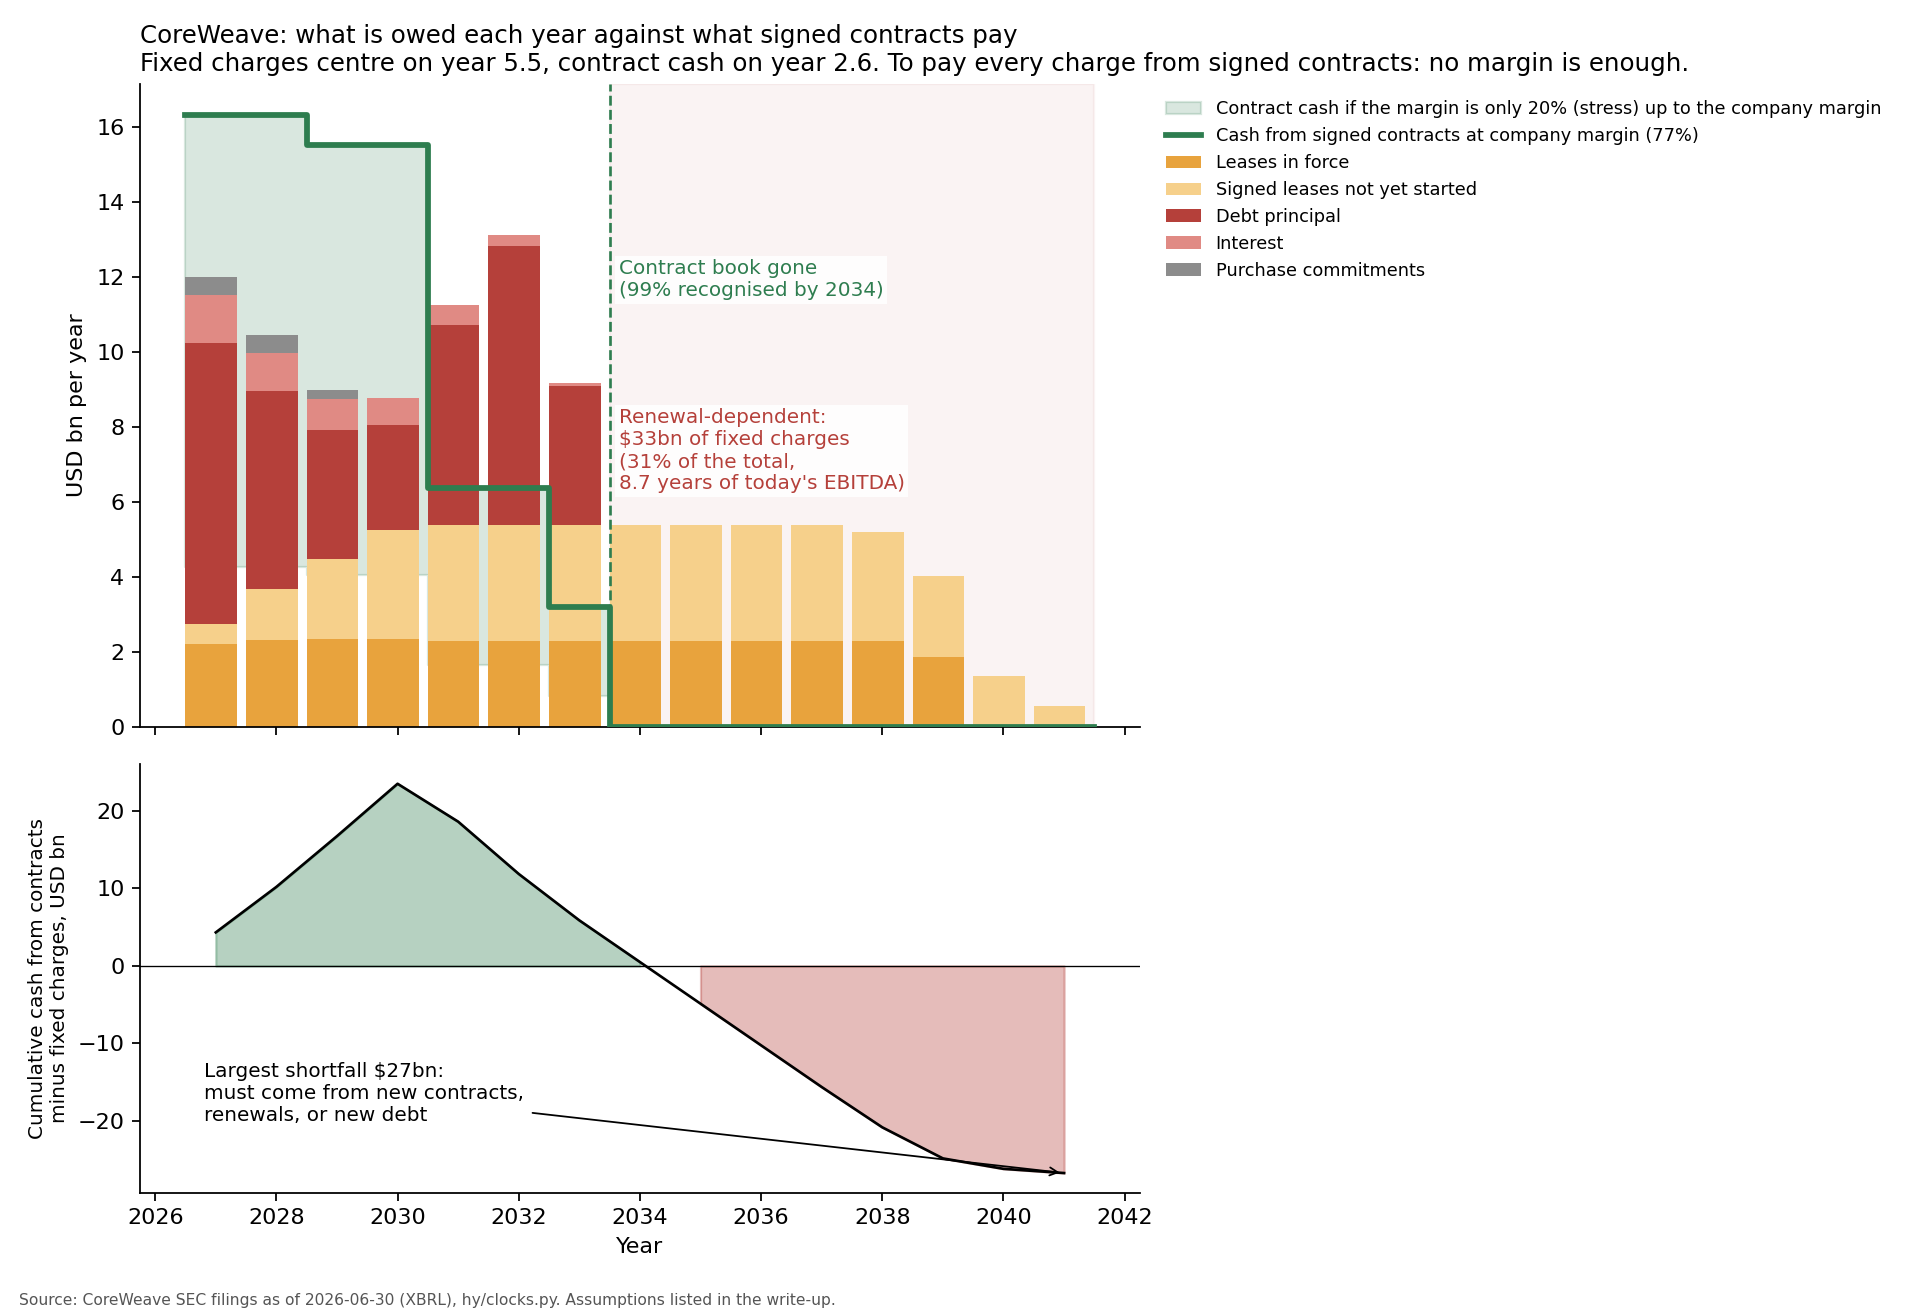
\includegraphics[width=\linewidth]{figures/clocks_CRWV.png}
\caption{Top: fixed charges each year (bars) against cash from signed contracts (green line at the company margin; green band down to a 20\% margin). Bottom: cumulative contract cash minus cumulative fixed charges. Red: years in which the charges have overtaken the contracts.}
\end{figure}

The fixed charges total \$112bn. Of this, \$29.1bn is rent on leases in force and \$35.5bn is rent on signed leases that start between 2026 and 2029, each for 7 to 16 years. Debt principal is \$35.6bn; interest and purchase commitments make up the rest.

The RPO is \$103.7bn. The 10-Q books 41\% in the next 24 months and 39\% in the 48 months after. It gives no timetable for the last 20\%.

The charges centre on year 5.3 and the contract cash on year 3.4. After the book runs off, \$27bn (24\%) is still due. That is 7.2 years of current EBITDA.

\begin{center}
\begin{tabular}{@{}lrr@{}}\toprule
CoreWeave & Contract cover & Largest shortfall \\\midrule
Base case (77\% margin) & 0.71 & \$33bn \\
Largest customer (36\% of revenue) does not pay & 0.45 & \$61bn \\
Add the excluded single-site lease (rent capped at \$14.7bn) & 0.63 & \$47bn \\\bottomrule
\end{tabular}
\end{center}

The concentration case is the downside that matters. One customer was 71\% of revenue a year ago and is 36\% now. The RPO by customer is not disclosed, so the case assumes the RPO splits like revenue.

The structure decides who absorbs a shortfall. \$31.4bn of the debt has recourse to CoreWeave. \$3.7bn sits in bankruptcy-remote subsidiaries, whose lenders hold \$18.2bn of assets as security (24\% of total assets). Those lenders are paid from those assets first. A parent unsecured creditor gets what remains.

\section{Oracle (10-Q, 31 August 2026)}

\begin{figure}[H]
\centering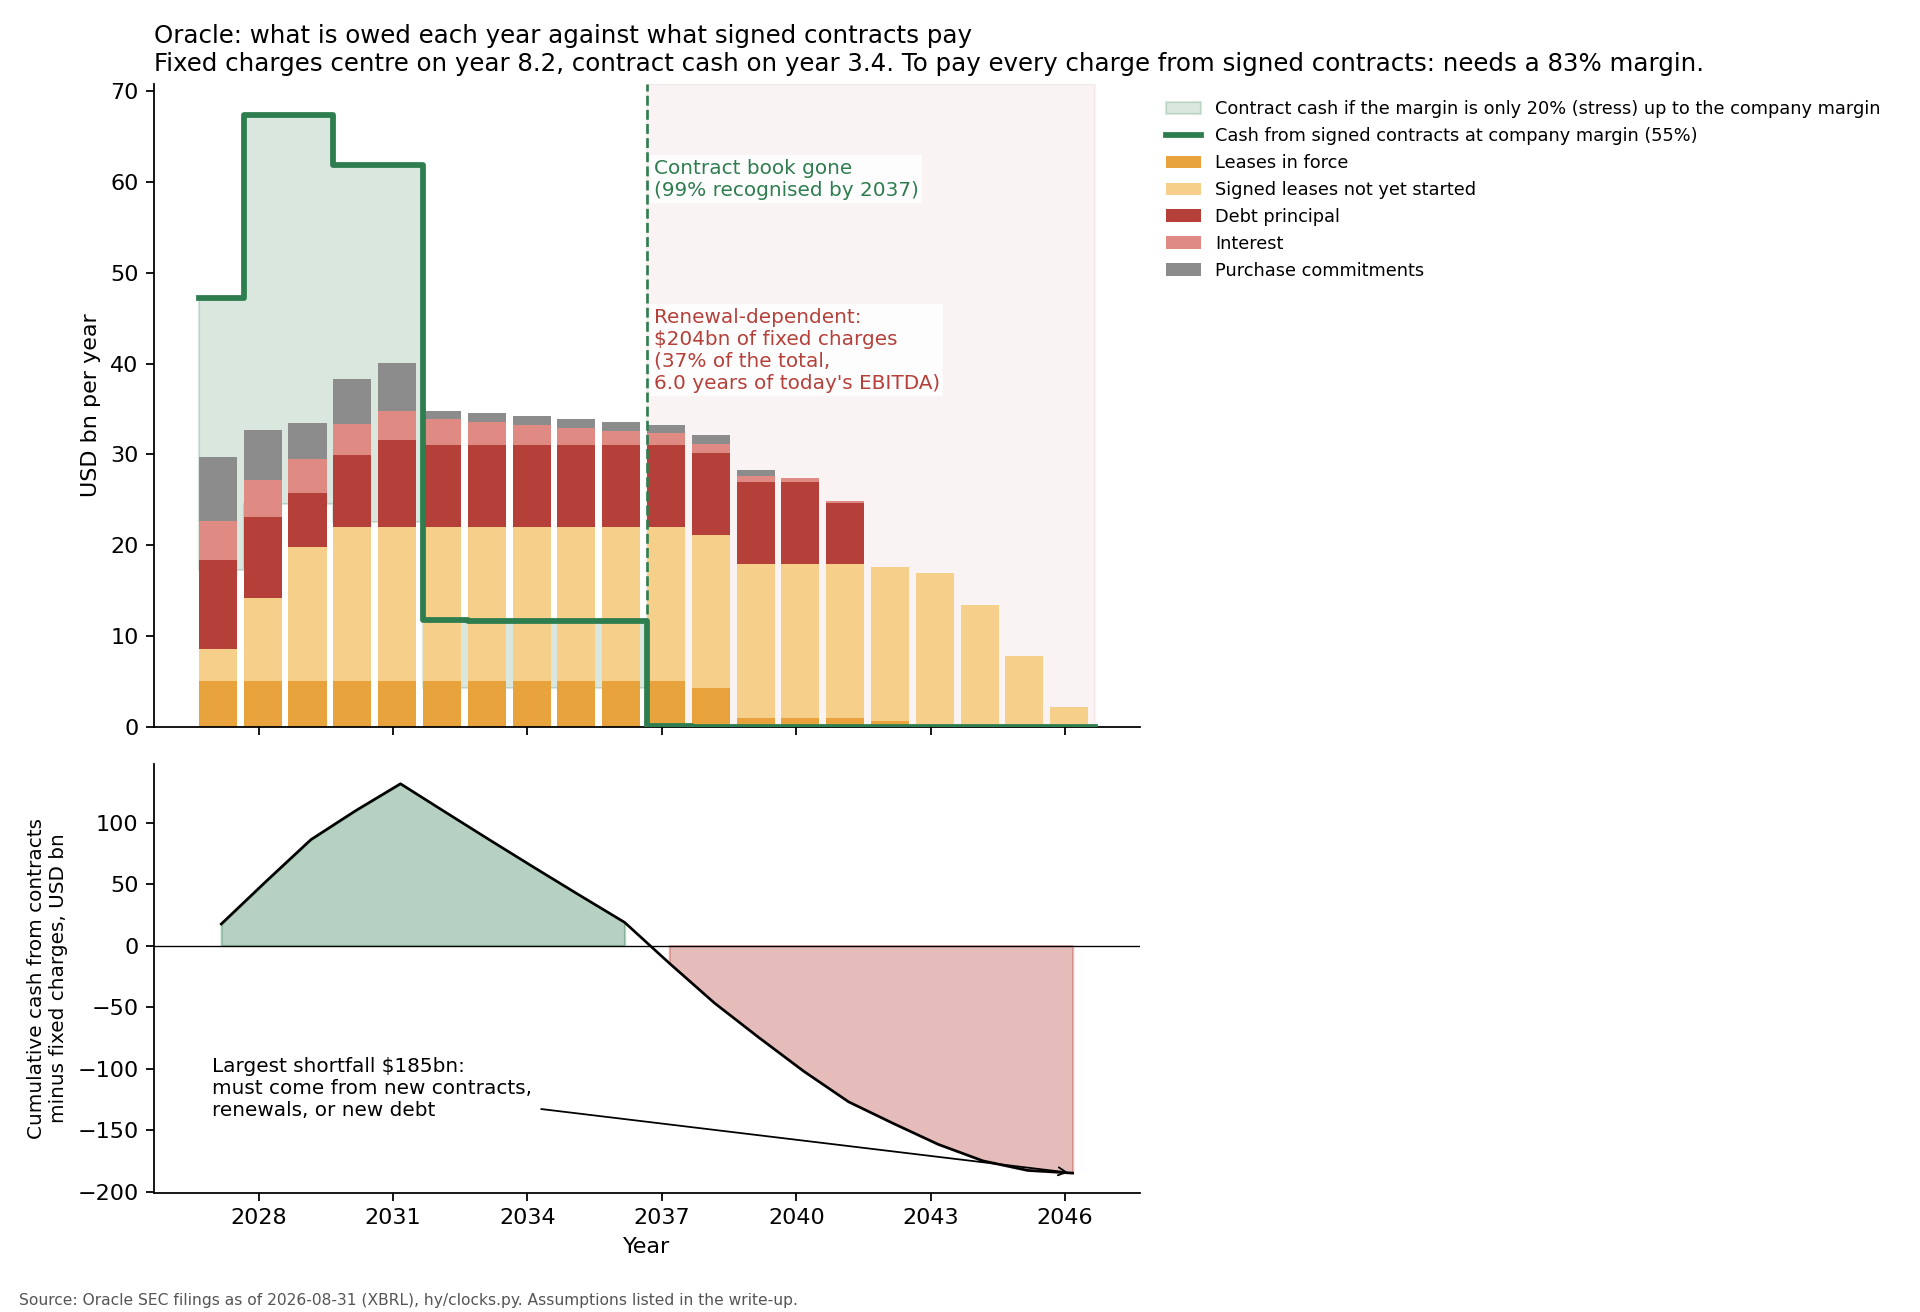
\includegraphics[width=\linewidth]{figures/clocks_ORCL.png}
\caption{Same layout as Figure 1. The green line applies Oracle's company-wide margin to a backlog that is mostly AI capacity, so read the band, not the line.}
\end{figure}

The fixed charges total \$559bn. The largest part is \$288bn of signed data-centre leases. They start between now and fiscal 2029 and run 15 to 19 years. Leases in force add \$63bn, debt principal \$130bn, and purchase commitments \$34bn; interest makes up the rest.

The RPO is \$664bn: 13\% in the next 12 months, 37\% in months 13 to 36, 34\% in months 37 to 60, and the rest after that.

The charges centre on year 8.2 and the contract cash on year 3.4. After the book runs off, \$205bn (37\%) is still due, or 6.0 years of current EBITDA. Oracle names no customer. S\&P estimates that about half of the backlog is OpenAI; the filing does not say so.

The company margin flatters the result. Oracle's margin of 55\% comes mostly from software. We do not know the margin on rented AI capacity. At 20\%, our stress case, signed contracts pay 24\% of the fixed charges.

\section{What would change the view}

\begin{center}
\begin{tabular}{@{}lrr@{}}\toprule
 & CoreWeave & Oracle \\\midrule
Breakeven margin $m^{*}$ & 1.08 & 0.84 \\
Contract cover at a 20\% margin & 0.18 & 0.24 \\
Contract cover at a 35\% margin & 0.32 & 0.42 \\
Contract cover at a 50\% margin & 0.46 & 0.59 \\
Contract cover at the company margin & 0.71 (77\%) & 0.65 (55\%) \\\midrule
Renewal-dependent share, last RPO books in 0.5 years & 29\% & 61\% \\
Renewal-dependent share, last RPO books in 2 years & 24\% & 55\% \\
Renewal-dependent share, last RPO books in 5 years & 10\% & 37\% \\\bottomrule
\end{tabular}
\end{center}

Two results do not depend on any assumption in the table. CoreWeave's breakeven margin is above 1. Oracle's is 29 points above its company margin.

One unknown moves the renewal share most: how fast the last part of the backlog is booked. For Oracle that part is 16\% of \$664bn. If it books fast, more of the 15-to-19-year rent has no contract behind it.

\section{The article, checked against the filings}

\begin{tabularx}{\linewidth}{@{}Xl@{}}\toprule
Claim in the article & Status \\\midrule
CoreWeave \$35.5bn of signed leases not started, 2026 to 2029, 7 to 16 years & \textcolor{good}{Confirmed} (XBRL and 10-Q text) \\
CoreWeave \$29.1bn of lease payments, 12-year average remaining term & \textcolor{good}{Confirmed} \\
CoreWeave \$103.7bn RPO, 41\% then 39\% & \textcolor{good}{Confirmed} \\
Top three customers 72\%; largest from 71\% to 36\% & \textcolor{good}{Confirmed} \\
Single-site lease capped at \$14.7bn, 393 MW not delivered & \textcolor{good}{Confirmed} \\
Oracle \$288bn of leases not started, 15 to 19 years & \textcolor{good}{Confirmed} \\
Ring-fenced assets of about \$20.8bn (44.5\% of net PP\&E) & \textcolor{bad}{Differs}: the 10-Q states \$18.2bn \\
CoreWeave RPO fully booked by month 78 & \textcolor{bad}{Not in the 10-Q}; the last 20\% has no timetable \\
Anthropic, OpenAI, and xAI commitment terms & Not in any filing (press reports, draft S-1) \\\bottomrule
\end{tabularx}

\section{Assumptions}
Each assumption is in \code{scripts/clock\_case.py} next to its source.
\begin{enumerate}
\item Signed leases that have not started begin at an even pace over the stated window. Each pays level rent over the midpoint term: 11.5 years for CoreWeave, 17 years for Oracle.
\item After the last stated year, rent continues at the last stated yearly amount until the stated total is paid: 8.3 more years for CoreWeave, 6.0 for Oracle.
\item Debt due ``thereafter'' is spread over 2 years for CoreWeave (its 2031 to 2032 maturities) and 10 years for Oracle. Oracle's schedule comes from its May 2026 10-K, moved forward one quarter. Interest is 9\% for CoreWeave and 4.5\% for Oracle on the balance that remains after each repayment. The model does not refinance any debt.
\item RPO after the last stated window books over 2 years for CoreWeave and 5 years for Oracle.
\item Contract cash left over in early years counts toward later charges. Capex and taxes take part of it in practice, so the largest shortfall is a lower bound.
\item The 20\% stress margin is our assumption. No filing gives a margin for rented AI capacity.
\end{enumerate}

\section{Rerun or extend}
\begin{itemize}
\item Run: \code{PYTHONPATH=. python3 scripts/clock\_case.py}. The script reads the latest filings from SEC XBRL, draws both figures, and writes one JSON per borrower to \code{data/raw/clocks/}, stamped with the filing's acceptance time.
\item Add a borrower: add an entry to \code{CASES} in that script.
\item Method: \code{docs/methodology.md} Section 4.7.
\item Decision record: \code{docs/decisions/}\allowbreak\code{2026-10-22-duration-mismatch.md}.
\item Tests: \code{tests/test\_clocks.py}.
\end{itemize}

\end{document}
